\chapter{Initial Process}
In this chapter the problem definition for Oasis is described.
An analysis of the requirements, received from the other groups in the multi project, are performed and from the analysis the Oasis system architecture has been derived.

\section{Problem Definition}
\label{sec:OasisProblemDefinition}
In the multi project a common problem definition have been stated, see Section \vref{sec:pdef}. The common problem definition is -- as stated -- to vogue for the individual groups. Therefore we have devised a problem definition for Oasis.
It is as follows:

\begin{quotation}
	\textit{How can we provide a set of tools, which can help develop applications for the GIRAF system?}
\end{quotation}

\section{Requirements}
Before the development can begin the requirements for the software must be analyzed.
The requirements stem from the multi project groups and the contact persons.
Examples of the requirements received can be seen in Appendix \vref{sec:timerreq} and \vref{sec:customerReq}.
\newpage
The derived informal requirements are:
\begin{itemize}
	\item Child profile handling
	\item Guardian profile handling
	\item Child and guardian relation handling
	\item Application specific profile setting handling
	\item Certificate handling
	\item Media handling
	\item Media access handling
	\item Media to media relation handling
	\item Department handling
	\item Department to subdepartment handling
	\item Profile to department relation handling
\end{itemize}

We have decided to develop a database and a library, which are to be used by GIRAF applications.
As an example of a GIRAF application, that uses the library and database, we will develop an administration application.

\section{System architecture}
\label{sec:OasisSystemArchitecture}
Oasis consists of three parts; The Oasis Local Db, the Oasis Lib, and the Oasis App. This is shown in Figure \vref{fig:systemArchitecture}.

The Oasis Lib handles application interaction with the Oasis Local Db, and every GIRAF application should be utilizing this library.
Another feature the Oasis Lib offers is the ability to handle synchronization between the Oasis Local Db and Savannah.

The last part is the Oasis App.
This application allows interaction with the Oasis Local Db through the Oasis Lib. 
Some of the features of the Oasis App are creation and removal of profiles and departments.
It also enables the user to handle relations between specific elements.

\begin{figure}
	\centering
		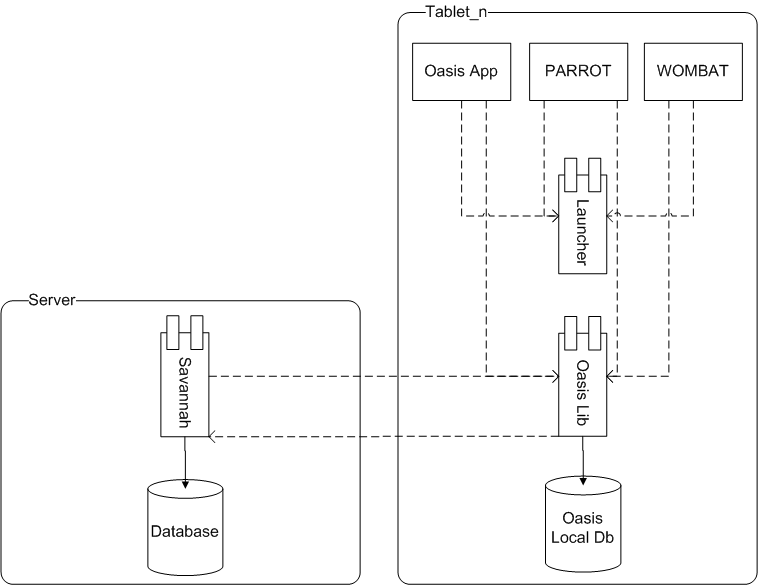
\includegraphics[width=\textwidth]{Images/Giraf_comp_pic_fix}
	\caption{The GIRAF sytem architecture.}
	\label{fig:systemArchitecture}
\end{figure}